\documentclass[tikz,border=8pt]{standalone}
\usepackage{amsmath}
\usetikzlibrary{arrows.meta,positioning,fit}

\begin{document}
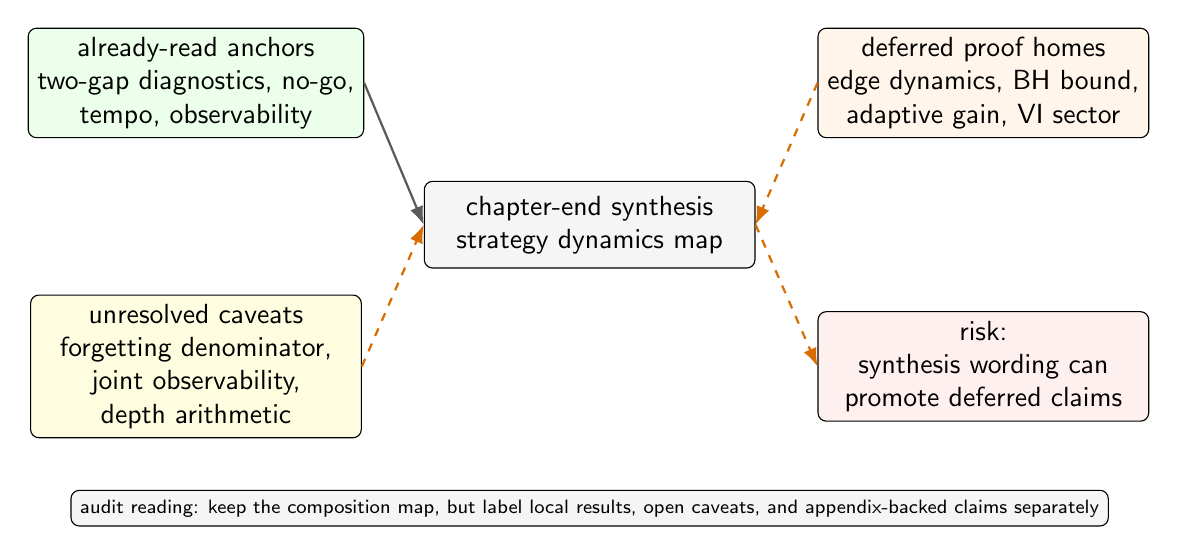
\begin{tikzpicture}[
  font=\sffamily,
  box/.style={draw, rounded corners=3pt, align=center, minimum width=42mm, minimum height=11mm, fill=white},
  note/.style={align=center, font=\sffamily\scriptsize},
  arrow/.style={-Latex, thick, draw=black!65},
  warn/.style={-Latex, thick, dashed, draw=orange!85!black}
]

\node[box, fill=gray!8] (hub) at (5,0)
  {chapter-end synthesis\\strategy dynamics map};

\node[box, fill=green!8] (read) at (0,1.8)
  {already-read anchors\\two-gap diagnostics, no-go,\\tempo, observability};
\node[box, fill=yellow!12] (caveat) at (0,-1.8)
  {unresolved caveats\\forgetting denominator,\\joint observability,\\depth arithmetic};
\node[box, fill=orange!8] (future) at (10,1.8)
  {deferred proof homes\\edge dynamics, BH bound,\\adaptive gain, VI sector};
\node[box, fill=red!6] (risk) at (10,-1.8)
  {risk:\\synthesis wording can\\promote deferred claims};

\draw[arrow] (read.east) -- (hub.west);
\draw[warn] (caveat.east) -- (hub.west);
\draw[warn] (future.west) -- (hub.east);
\draw[warn] (hub.east) -- (risk.west);

\node[note, fill=gray!8, draw, rounded corners=3pt, minimum width=92mm] at (5,-3.6)
  {audit reading: keep the composition map, but label local results, open caveats, and appendix-backed claims separately};

\end{tikzpicture}
\end{document}
